\section{Цель работы}
\begin{enumerate}
    \item Изучение основных характеристик свободных затухающих колебаний
\end{enumerate}

\section{Объект исследования}
Объект исследования - затухающие свободные колебания, возникающие в колебательном контуре.

\section{Метод экспериментального исследования}
Многократное прямое измерение колебаний в колебательном контуре.

\section{Рабочие формулы и исходные данные}
\begin{enumerate}
  \item Логарифмический декремент
    \( \lambda = \frac{1}{n} \ln \frac{U_i}{U_{i+n}} = \beta T = \frac{R}{L} = \frac{\pi}{\sqrt{1/LC - (R/2L)^2}} \)
  \item Полное сопротивление \(R = R_\text{м} + R_0 \)
  \item Зависимость логарифмического декремента от сопротивления при малых затуханиях
    \( \lambda \approx \pi R \sqrt{C/L} \).
    Тогда
    \( L \approx \frac{\pi^2 R^2 C}{\lambda^2} \).

  \item Период затухающих колебаний:
    \( T = \frac{2 \pi}{\sqrt{1/LC - (R/2L)^2}} \)

  \item Добротность контура для малых затуханий:
    \( Q = 1/R \sqrt{L/C} = \frac{2 \pi}{1 - e^{-2 \lambda}} \).

  \item Критическое сопротивление: \( R_{кр} = 2 \sqrt{L/C} \).

  \item Формула Томпсона:
    \( T = 2 \pi \sqrt{L C} \)
\end{enumerate}

\section{Измерительные приборы}
\begin{table}[ht]
    \centering
    \begin{tabular}{| c | c | c | c | c |}
        \hline
        \textnumero п/п & Наименование & Тип прибора & Используемый диапазон & Погрешность \\
        \hline
        1 & Осциллограф & цифровой & \(K_y = 0.2 \pm 1\,\text{В}\), \(K_x = 10\,\text{мс} \) & \( K_\text{откл} = \pm 3\% \) \\
        \hline
    \end{tabular}
    \caption{Измерительные приборы}
\end{table}

\section{Схема установки}
\begin{figure}[ht]
    \centering
    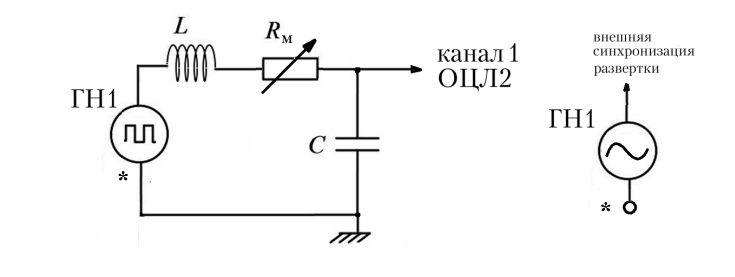
\includegraphics[width=0.9\textwidth]{./img/scheme.png}
    \caption{Схема установки}
\end{figure}
